
\subsubsection{Networks and
Distributed Systems}\label{ict:cns:schoenwaelder} \index{Sch\"onw\"alder,
J\"urgen}

\paragraph{Research Team}
J\"urgen Sch\"onw\"alder (Professor), Ha Manh Tran (PhD Student), Vlad Balan (MSc
Student), Mat\'u\v{s} Harvan (MSc Student), Vladislav Marinov (MSc Student)\\

Computer networks such as the Internet continue to change many aspects
of our daily life. The networks and protocols research group carries
out research related to Internet protocols, with strong relationships
to work undertaken by the Internet Engineering Task Force (IETF), an
organization responsible for Internet protocol standardization, and
the Internet Research Task Force (IRTF), an organization responsible
for longer-term research related to Internet protocols.

\paragraph{Highlights}

The operation of increasingly complex communication networks requires
supporting systems, so called network management systems.  Network
management protocols and associated data definitions have been
developed and standardized over the last decade to support open,
vendor-neutral access to management and control information.  While
some of these technologies are in wide-spread usage, there is little
information how the underlying protocols are utilized and what the
specific characteristics of network management interactions are. As a
consequence, there are no well accepted models which can be used to
analyze the impact of protocol changes.

\begin{figure}[ht]
  \begin{center}
     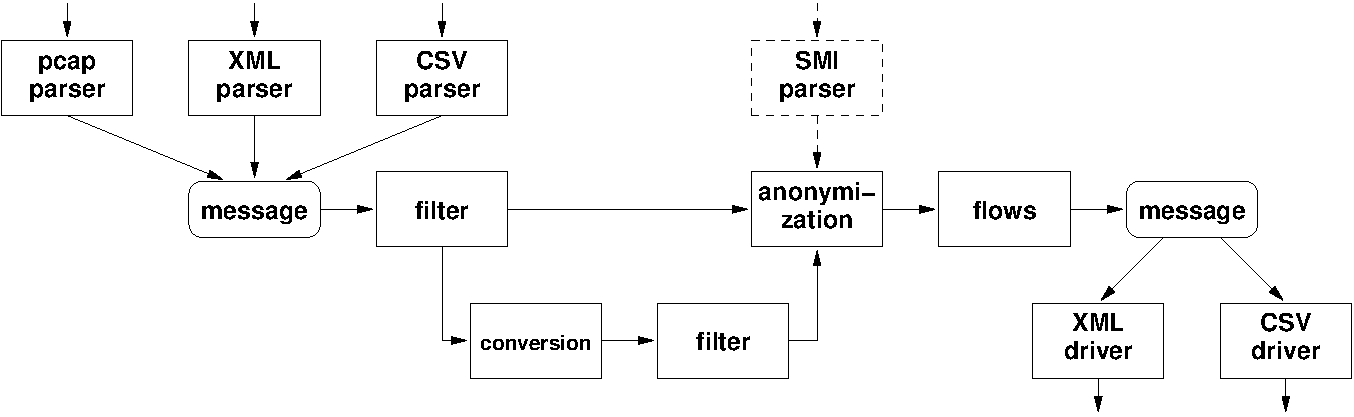
\includegraphics[width=\hsize]{schoenwaelder-tools}
  \end{center}
  \caption{Data flow within the \texttt{snmpdump} tool}\label{fig:snmpdump}
\end{figure}

A larger empirical study has been started in 2006 where we collect network management
packet traces from operational networks. This study is carried out in collaboration with
international research groups and supporting operators in order to obtain traces from live
networks. Based on an anonymization algorithm developed in 2005 \cite{HS06}, our group has
designed and implemented a tool chain (Fig.~\ref{fig:snmpdump}) for the analysis of
network management traffic traces \cite{PSHSM07}. Further research is ongoing to develop
analysis algorithms able to infer high-level management operations from observed primitive
protocol operations.

\begin{figure}[ht]
  \begin{center}
     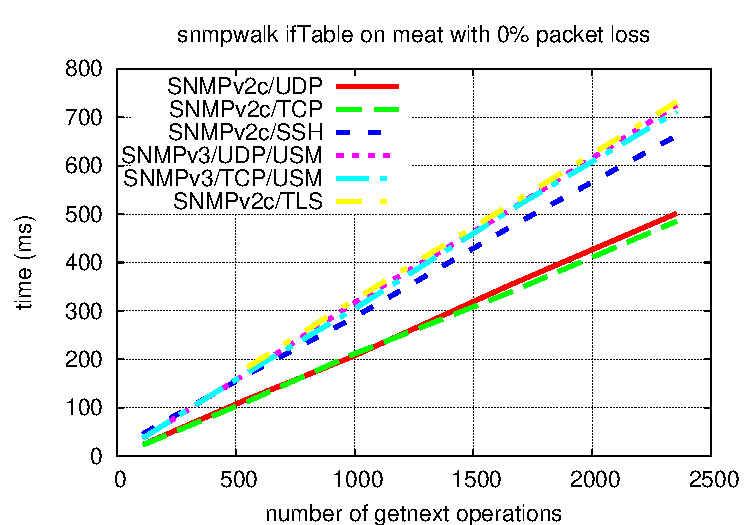
\includegraphics[width=\hsize]{schoenwaelder-sec}
  \end{center}
  \caption{Latency of SNMP/SSH and SNMP/TLS}\label{fig:sshtls}
\end{figure}

A related activity concerns the security of network management
interactions (Fig.~\ref{fig:sshtls}). We have prototyped and analyzed
a security extension proposed for the SNMP which leverages transport
layer security protocols such as SSH or TLS \cite{MS06}. This work is
related to standardization efforts undertaken by the Integrated
Security Model for SNMP (ISMS) working group of the IETF.

\begin{figure}[ht]
  \begin{center}
     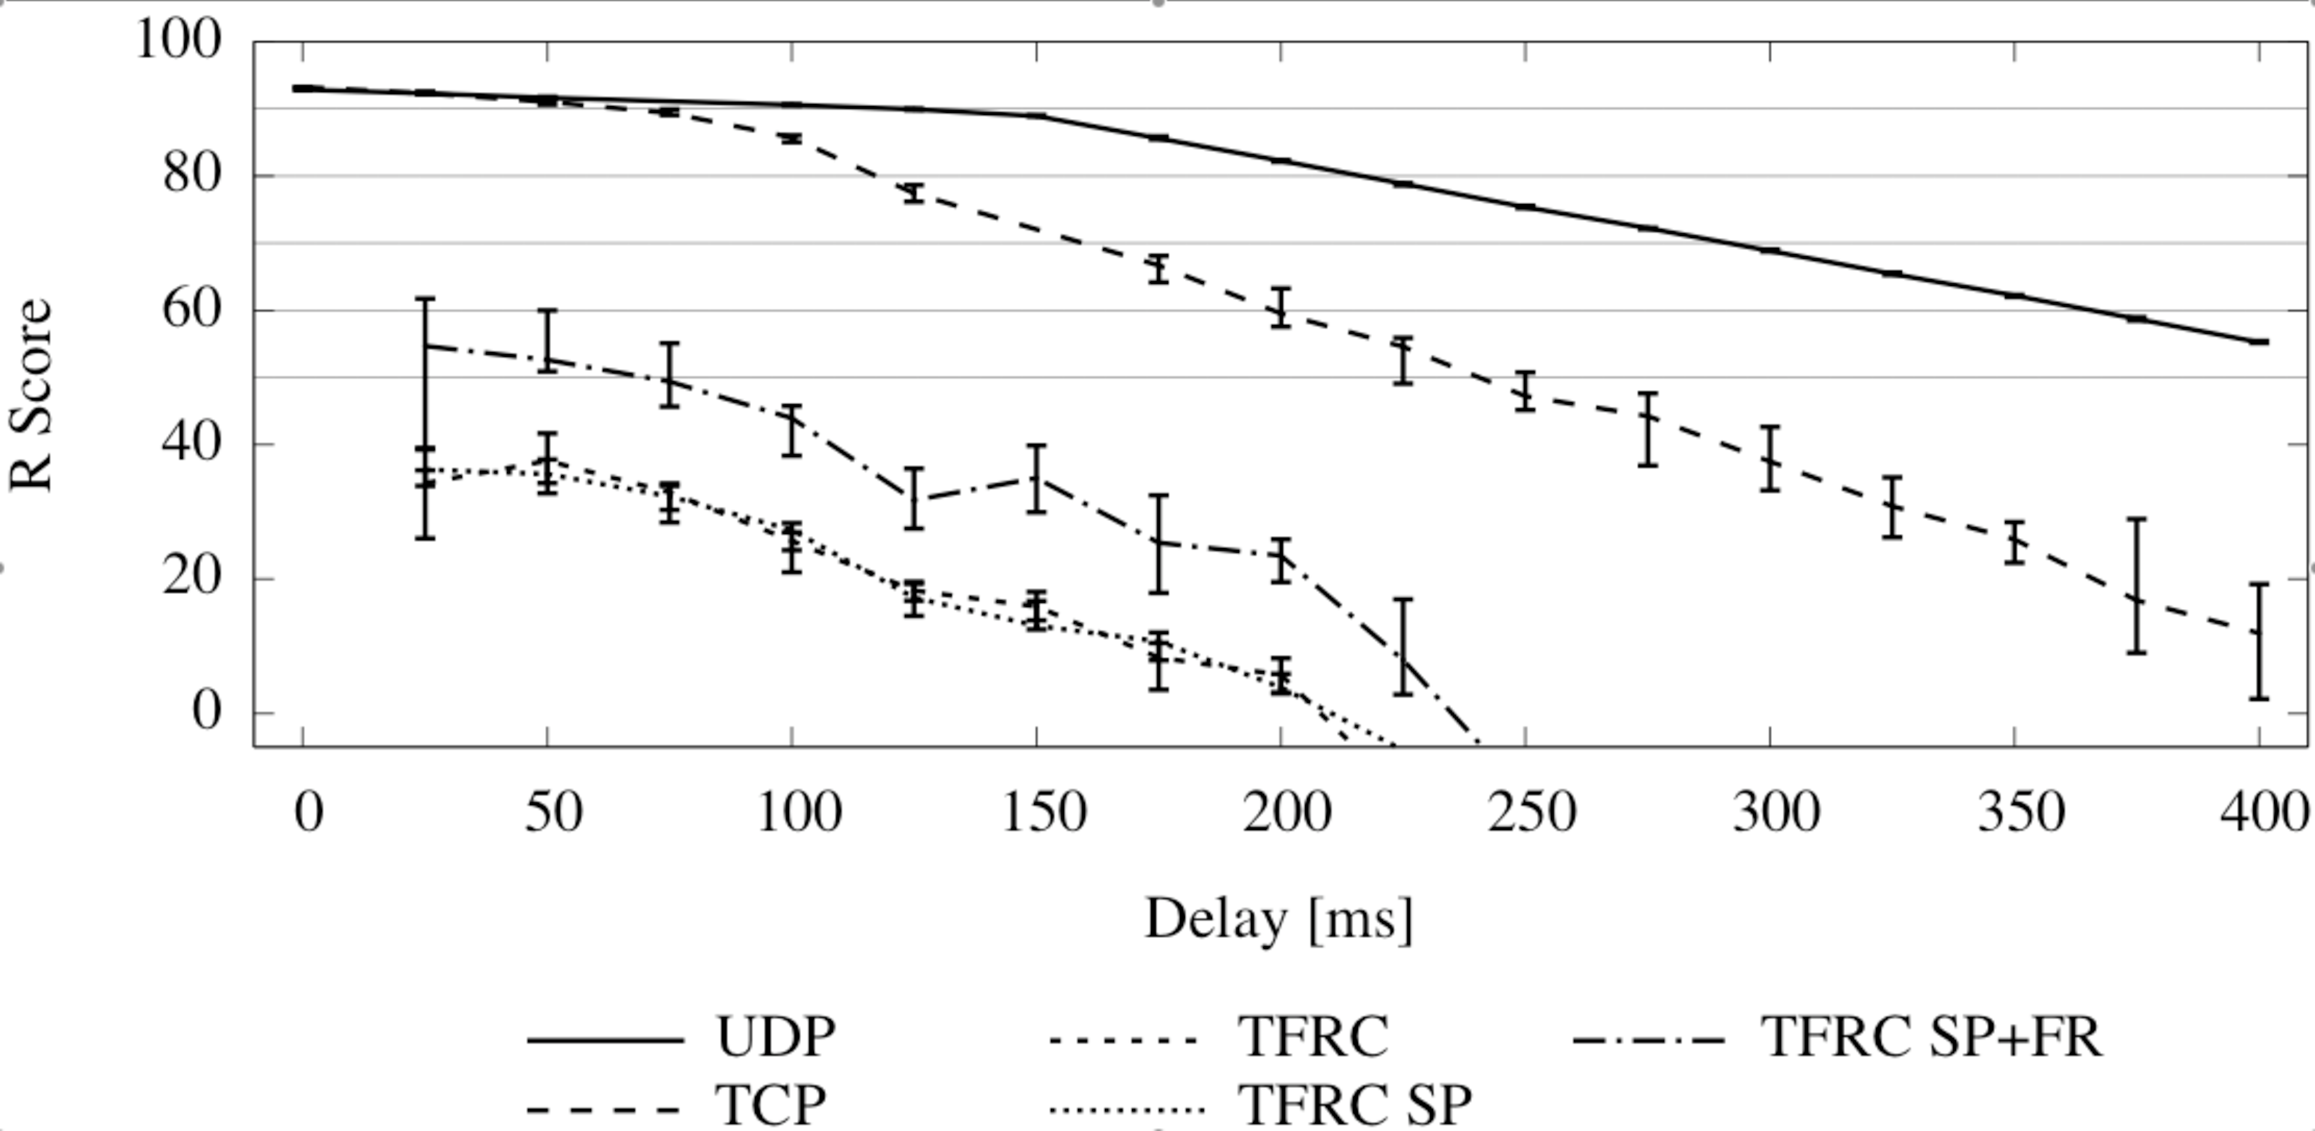
\includegraphics[width=\hsize]{schoenwaelder-dccp}
  \end{center}
  \caption{R scores for G.711 over DCCP}\label{fig:sshtls2}
\end{figure}

Finally, we have conducted research on the performance of voice stream
transmission over the new Data Congestion Control Protocol (DCCP)
being standardized by the IETF \cite{BENB07}. This work was carried out in
close collaboration with NEC C\&C Research in Heidelberg, Germany.


\penalty -50
\paragraph{Organization}\nobreak
% list the (research) events you have organized, if any,
\begin{enumerate}
    \item Editorial board member of the IEEE electronic Transactions on
          Network and Service Management
    \item Guest Co-Editor of a special issue on Peer-to-Peer
          Technologies in Network and Service Management of the
          Journal of Network and Systems Management
    \item Program Committee member of NOMS 2006, ACC 2006, DSOM 2006,
          IM 2007, ICCC 2007 NSO, SASO 2007, AIMS 2007
    \item Reviewer IEEE Communications Magazine, IEEE Transactions on
          Software Engineering, Springer Journal of Network and
      Systems Management
    \item Co-Chair of the IETF ISMS working group
    \item Member of the Security Directorate of the IETF
    \item Chair of the Network Management Research Group (NMRG) of the IRTF
    \item Chair of the 19th NMRG workshop on ``Promise Theory and New
          Approaches to Distributed Management'', KTH, Stockholm, January
          2006
    \item Chair of the 21st IRTF NMRG workshop on ``Future Direction
          of Network and Service Management Research'', SurfNet,
          Utrecht, October 2006
    \item Dissemination Activity Leader / Member of the Executive
          Committee of the EMANICS Network of Excellence
\end{enumerate}

\paragraph{Collaborations}
\begin{enumerate}
    \item {\sl University of Twente, The Netherlands}\\
          Prof.\ Aiko Pras\\
          Network Management, Traffic Measurements
    \item {\sl INRIA Lorraine, France}\\
          Prof.\ Olivier Festor\\
          Scalability of Management Protocols
    \item {\sl NEC C\&C Research}\\
          Dr.\ Lars Eggert\\
          Analysis of Voice over the Datagram Congestion Control Protocol
    \item {\sl NEC C\&C Research}\\
          Dr.\ J\"urgen Quittek\\
          Integrated Security Model for the Simple Network Management Protocol (SNMP)
    \item {\sl Huawei}\\
          David Harrington\\
          Architectural Models for Internet Management Protocols
    \item {\sl IEEE Project 802}\\
          Tony Jeffree\\
          SNMP over IEEE 802 Networks
\end{enumerate}

\paragraph{Grants}
\begin{enumerate}
    \item Funded by EU-IST NoE,  \emph{ ``EMANICS (EU Network of Excellence for the Management
      of Internet Technologies and Complex Services)''}, (January 2006 - December
      2009)
\end{enumerate}

%\paragraph{Awards, Prices}
%\begin{enumerate}
%\item IM 2005 Distinguished Experts Panel (invited panelist)
%\end{enumerate}

%\paragraph{Publications}

%\begin{description}
%  \item[Conference Proceedings]
  \nocite{HS06} \nocite{MS06} \nocite{BENB07}
  \nocite{PSHSM07} \nocite{DKPM07}
  %\item[Books/Collections]
  \nocite{Sch07}
 % \item[Standards]
  \nocite{RFC4789}
%\end{description}
%\end{document}
%%% Local Variables:
%%% mode: latex
%%% TeX-master: "report"
%%% End:
